\chapter{\ca{Implementation}}
\renewcommand{\baselinestretch}{\mystretch}
\label{chap:Impl}
%\setlength{\parindent}{0pt}

\PARstart{\ca{S}}{\ca{everal}} \ca{%
implementations of various portions of the final optimised controller application were developed independently, so that each portion can be verified working before integration. The implementations were developed as the following steps:
}

\begin{enumerate}[noitemsep,leftmargin=4cm]
  \item[Qt2 demo:] A controller specific application using C++ with Qt2-based GUI, to test the performance of the NP1380 platform and showcase an interactive application design.
  \item[\texttt{VixenLinky}:] C\# implementation of a controller specific application, for use as the references of the optimal performances on different platforms.
  \item[Playback engine:] Integrate the sequence decoding routine from \texttt{VixenLinky} to the Vixen application as a separate playback engine.
  \item[\texttt{VixenConsole}:] A command-line interface (CUI) version of the Vixen application, but with only minimal functionalities and a working playback engine for embedded platforms.
  \item[Video transcoding:] Various programs for video processing, integrated into the playback engine for video format support.
\end{enumerate}

\clearpage

\section{\ca{Qt2-based} implementation}

A GUI application dedicated to the \texttt{TCPLinky} controller was developed using C++ as \ca{a user-friendly alternative implementation} showcase. This application was developed specific to the Noah NP1380 platform listed in \sref{sec:systems}. This device is a handheld embedded device based on a 10 years old SoC chip, originally designed for educational use \ca{such as electronic dictionaries}. Fortunately, this devices uses Linux system and Qt2 as GUI. Therefore, it is possible to test Vixen application on this low-end platform.

\begin{figure}[t]
  \centering
  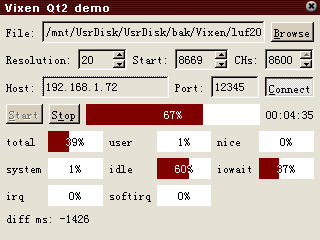
\includegraphics[width=0.45\textwidth]{Figs/vixen_noah.png}%
  \caption{\footnotesize Screenshot of Vixen Qt2 demo on Noah NP1380}
  \label{fig:vixen_noah}
\end{figure}

\fref{fig:vixen_noah} shows a screenshot of the dedicated application. The method of performance profiling through statistic files in proc file system was also tested. These smaller progress bars at the lower half of the application shows percentages of CPU time spent on different tasks, such as user space applications, kernel mode and interrupt handling. Most of the time only less than $50 \%$ CPU time was used for this controller application, \ca{indicating that} even this low-end device is capable of handling thousands of lighting channels.

\section{Minimal C\# implementation}

To set up a reference baseline for optimal performance, sequence rendering application \ca{named \texttt{VixenLinky} was developed. It was implemented using C\#, takes} the same \ca{``Raw''} sequence data \ca{format}, but \ca{supports} only the \texttt{TCPLinky} controller developed in \sref{sec:tcplinky}. \ca{It was} implemented as \ca{simply} as possible without all intermediate layers \ca{and module loading routines}, but still \ca{using} a threading structure \ca{identical to} the original Vixen application. \ca{The source code for controlling the \texttt{TCPLinky} controller} was ported directly from the original Vixen application \ca{to ensure compatibility and similarity}.

With this program, the \ca{ideal} performance \ca{of the new playback engine} on each platform can be measured. The \ca{remaining performance limitation factors are} sequence loading performance and controller update speed. Therefore, options to unlimit the update interval of both sequence loading and controller update were added separately \ca{for the measurements of maximum update rates}.

\fref{fig:vixenlinky_noah} shows an example of performance data gathered on the Noah NP1380 platform through \texttt{VixenLinky} using \ca{the exported test sequence}. The refresh rates of both playback and controller \ca{were} very stable around \ca{the configured} 50 fps. The CPU usage \ca{peaked} at $60.0 \%$\ca{,} while most of the time it \ca{was} distributed around $20.0 \%$ and $30.0 \%$ (first and third quartiles).

\begin{figure}[!t]
  \centering
  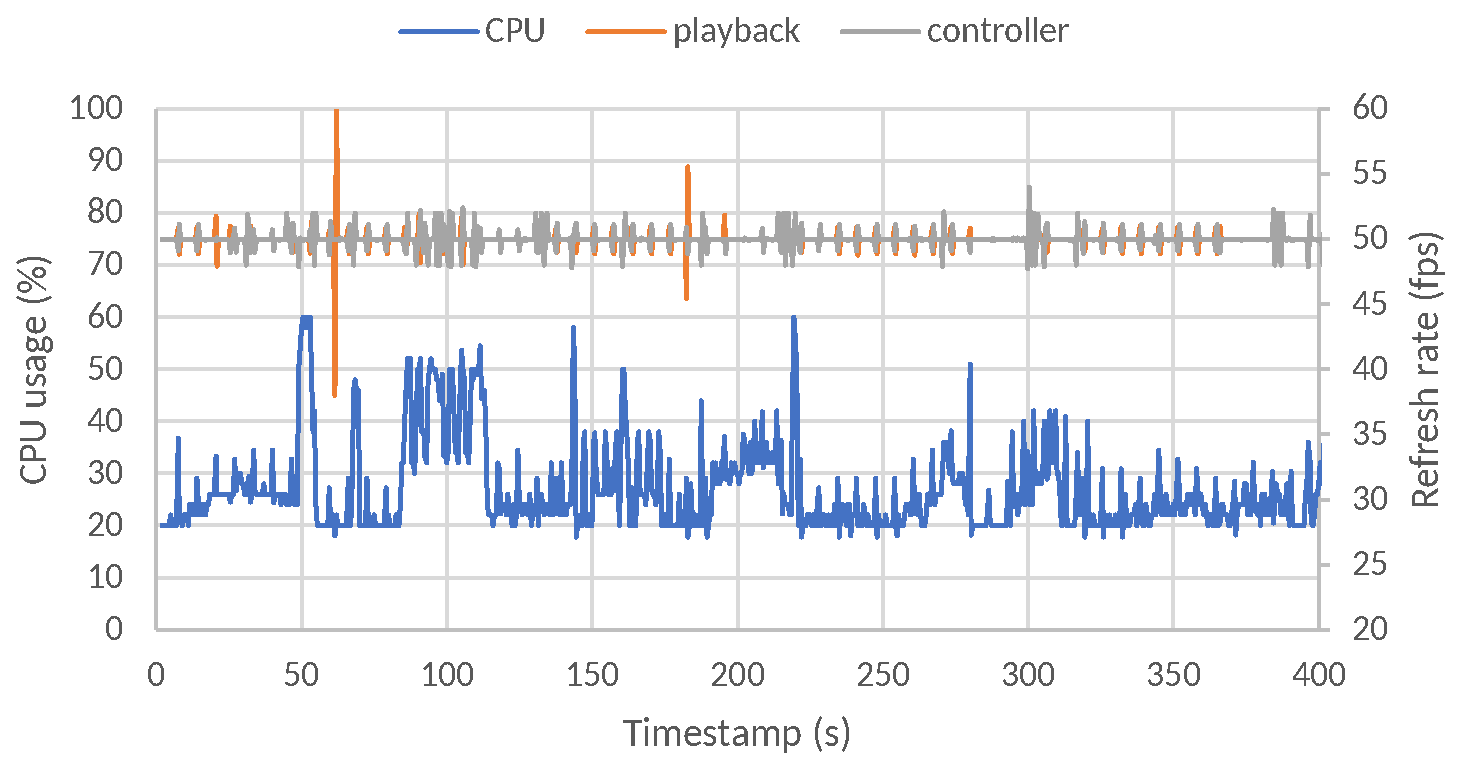
\includegraphics[width=0.8\columnwidth]{Figs/vixenlinky_noah.eps}
  \caption{\footnotesize Performance of \texttt{VixenLinky} on Noah NP1380}
  \label{fig:vixenlinky_noah}
\end{figure}

\section{Playback engine}

\section{Implementation}

After \ca{verifying} the ability \ca{to load and render} the exported lighting \ca{sequences} by controller specific \ca{applications}, the C\# code for loading exported sequence \ca{from \texttt{VixenLinky}} was integrated into Vixen application as a separate playback engine.

Several code branches were added to switch between the original execution engine and the new playback engine. The execution engine was still used as the default engine to simplify status checking and support the sequence editor. The playback engine will be switched to \ca{only if an exported sequence was loaded to it and started rendering}.

The playback engine starts by reading the exported network XML file. To simplify the process, \ca{an} XML object serialiser was used to interpret \ca{and store} the XML \ca{data structure} to a similarly structured C\# object for later access. The information \ca{read} from XML will be used to determine controller channel mapping, update interval and optional audio media file. To further reduce \ca{matching} overhead, the controller names will be looked up and converted to their unique ID (GUID) \ca{instead}. The optional audio media file was supported by utilising the same audio media functions from original execution engine.

All preview, element and filter updates were skipped in the playback engine. The translation layers were skipped, since the sequence data is already specific to the controllers. However, in order to match the existing interface of controller modules, \ca{segments of sequence data frame buffer} still need to be copied again \ca{as command batches for each controllers}, incurring some unnecessary overhead.

The structure of update management was also changed. \ca{In the original execution engine}, the application updates \ca{data buffers} from \ca{controller update requests}, which requires the use of mutex \ca{locks to coordinate} data \ca{accesses} between controller threads. With a configuration \ca{consists} of multiple controllers, potential lock contention of the mutex can also incur some overhead. \ca{To address this issue, another} thread dedicated to sequence loading was \ca{added} to the playback engine, \ca{similarly} to the structure of controller specific implementations. In this way, only the sequence loading thread may update the channel data buffer, \ca{removing} the need of mutex \ca{locks}.

\cmt{Add graph to explain the change}

One major drawback of using the playback engine is that the \ca{exported} data cannot be mapped back to element states yet\ca{, which is essentially the reverse of export}. Therefore, editing the \ca{exported} sequence using the built-in editor and the preview output were not supported.

\section{Integration}

A simple control dialog was added as a menu entry for the \ca{new playback} engine, as shown by \fref{fig:vixen_playback}. More complex and user-friendly UI design is possible, however, due to limited time \ca{constraints} this control dialog should be sufficient for this project and proof of concept.

\begin{figure}[t]
  \centering
  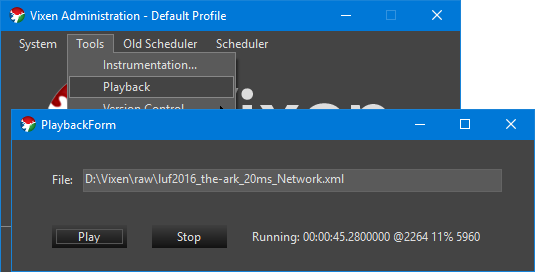
\includegraphics[width=0.8\columnwidth]{Figs/vixen_playback.png}
  \caption{\footnotesize Screenshot of the playback engine control dialog}
  \label{fig:vixen_playback}
\end{figure}

The playback control was also integrated \ca{as a new type of action into the} built-in schedulers. It can therefore be scheduled to execute at specific \ca{times with different sequences}, possibly \ca{together with other existing actions including} schedules using the original execution engine. The new playback engine does not need additional pre-process for show schedules, \ca{thus} can be directly started within seconds.

\section{Performance}

\fref{fig:playback} shows the performance of the \ca{new} playback engine \ca{on the same Microsoft Windows-based platform} using \ca{an exported} ``Raw'' sequence. At the first and the last few seconds, the playback engine stopped, the original execution engine was used instead during idle state. However, the execution engine still uses around $30 \%$ of CPU time during idle. But as soon as playback started, CPU usages drops to around $6 \%$ with stable refresh frame rates.

\begin{figure}[t]
  \centering
  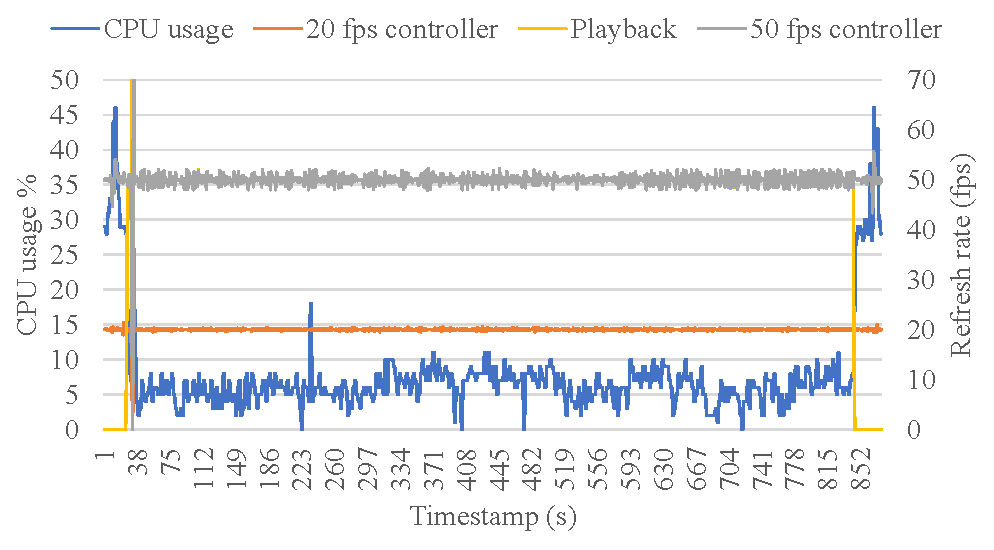
\includegraphics[width=0.8\columnwidth]{Figs/playback.eps}
  \caption{\footnotesize Performance of the new playback engine on Microsoft Windows}
  \label{fig:playback}
\end{figure}
